\chapter{Related Work}
In this section, we will have a look at what are the existing approaches and what efforts
have been taken by others to allow languages to interact.

\section{JVM/CLR Language Inter Operations}

We first look into the Microsoft .NET's Common Language Runtime (CLR) and the Java Virtual Machine (JVM). Both these systems allow users to program in different languages allowing multi-language support. 

\subsection{CLR}

\begin{figure}[h]
	\begin{center}
		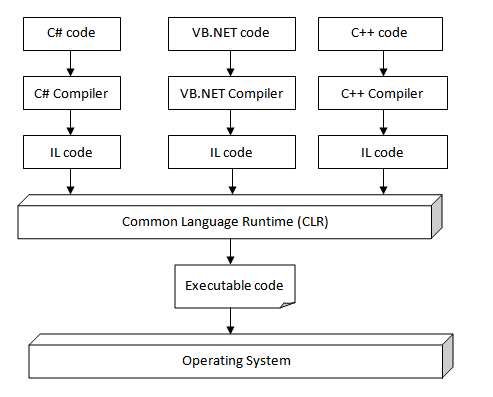
\includegraphics[width=\linewidth]{./images/clrArchitecture.png}
	\end{center}
	\caption{Common Language Runtime : Architecture \cite{clrarchitecure}}
	\label{fig:clrarchitecture}
\end{figure}

The Common Language Runtime (CLR) is a virtual component of Microsoft's .NET framework. It provides runtime environment, which runs the code from various languages and also provides environment, which makes software development process very easy \cite{Kennedy:2001:DIG:381694.378797}. Figure \ref{fig:clrarchitecture} shows the architecture of CLR.


Tools and compilers expose the CLR's functionality, so that you can take advantage of this common language runtime's managed execution environment. The code written to target the common language runtime is known as managed code. This code can be benefited from features such as a cross-language integration, cross-language exception handling, versioning, and security by providing simplified way for component interactions \cite{commonlanguageruntime}.

The compiler converts the source code into the Intermediate Language Code (IL code). IL code is CPU independent instructions that can be converted into the native code. At the runtime, The CLR's Just In Time (JIT) compiler converts this IL code into native code.

Compilers and tools able to produce the output consumed by the CLR, because, format of metadata, type systems are defined by the public standard called the ECMA Common Language Infrastructure \cite{Gough:2001:CNC:559569}.

The Compiler emits metadata describing members, types, and references in your managed code to insure common language runtime provides services to managed code. This metadata is used to load and locate classes, load instances in memory, generate native code, enforce security \cite{Gough:2001:CNC:559569}.

Achieving even slight levels of language interoperability is pretty difficult because of the wide variation in programming language features, and implementations. The CLR makes it easy to build components, and application whose objects can interact with each other across the languages. Code written in different languages can be integrated, their behavior is tightly integrated. For example, the class written in one language can be derived from the class written in other language and can call method of the class it is derived from. We can also pass instance of the class (Object) from one language to another. This is possible because language compilers, and tools uses common type system provided by CLR and they follow the CLR’s standard rule for defining, creating, and pertaining types \cite{Kennedy:2001:DIG:381694.378797}.


CLR provides following benefits: 

1) Language inter-operation ability.

2) Performance enhancements.

3) Garbage Collection.

4) Support for exception handling.

\subsection{JVM}

The Java programming language \cite{Gosling:1996:JLS:560667} implementation compiles to Java virtual machine language (JVML) \cite{Lindholm:2014:JVM:2636992},  also, known as Java-byte code. JVML is stored as java class files. It is either interpreted or compiled Just-In-Time (JIT) to native code by Java Virtual Machine (JVM). JIT allows efficient code as it is tailored as per the processor. Using such intermediate language provides many benefits \cite{clrspecification}. Languages supported by JVM compiles to common byte-code, which helps in language interoperability.

Singer, discusses about difference between JVM and CLR \cite{Singer:2003:JVC:957289.957341}.

\section{Java Scripting APIs}

After Java 6, Java supports incorporating code written in scripting languages directly in the Java. It enables developers to access their code written in scripting language directly in the Java applications. It began new generation of multi-language application called as polyglot applications (where the Java language can work together with other scripting languages). \cite{Juneau2017}

Developers were able to construct Java applications containing scripts developed in languages like JavaScript and Python. It uses JavaScript engine called Rhino \cite{rhinojava} in Java 6, which is replaced by Nashorn \cite{nashornjava} from Java 7. It is an implementation of the JavaScript engine, built entirely in the Java. It contains full support for the JavaScript \cite{Juneau2017}.


This scripting functionality is provided by the javax.script package. The package contains very simple and small APIs for accessing JavaScripts. Scripting APIs are accessible through scriptEngineManager class. scriptEngineManager objects can search for script engines by means of jar file service detection mechanism.

According to the Java documentation \cite{javascripting} Way to access nashorn engine in the Java application:

1.	Import the javax.script package.

2.	Instantiate a ScriptEngineManager object.

JavaScripting APIs can be accessed through the ScriptEngineManager class. A ScriptEngineManager object instantiates ScriptEngine objects. It also maintains a global variable values shared by API. 

3.	Obtain instance of ScriptEngine from the manager with getEngineByName() method.

getEngineByName() method takes one string parameter with name of the script engine. To obtain instance of the nashorn engine pass “nashorn”. We can also use one of the following arguments "ecmascript", "ECMAScript", "Nashorn", "JavaScript", "javascript", "js", "JS".
 
After, we have the Nashorn engine instance, we can use to embed scripts in our Java application. Let's see some of the examples, which show the use of Nashorn:

\textbf{Example 1 - Evaluating a statement}

Figure \ref{fig:nashornevalastatement} shows the example, which can evaluate "Hello world !" using Nashorn.

\begin{figure}[ht]
	\begin{lstlisting}
	import javax.script.*;
	
	public class EvaluateScript {
	 public static void main(String[] arguments) throws Exception {
	  ScriptEngineManager engineManager = new ScriptEngineManager();
	  ScriptEngine eng = engineManager.getEngineByName(``nashorn'');
	
	  // evaluate JavaScript code
	  eng.eval(``print(`Hello, World')'');
	 }
	}
	\end{lstlisting}
	\caption{Evaluating a statement: Nashorn}
	\label{fig:nashornevalastatement}
\end{figure}

In the example shown in Figure \ref{fig:nashornevalastatement}, the script engine calls the eval() method and executes JavaScript string passed as an argument to eval() function. 

\textbf{Example 2 - Evaluating a JavaScript file}


\begin{figure}[ht]
	\begin{lstlisting}
	import javax.script.*;
	
	public class EvalFile {
	 public static void main(String[] arguments) throws Exception {
	  ScriptEngineManager engineManager = new ScriptEngineManager();
	  ScriptEngine eng = engineManager.getEngineByName(``nashorn'');
	
	  eng.eval(new java.io.FileReader(``script.js''));
	}
	}
	\end{lstlisting}
	\caption{Evaluating a JavaScript file: Nashorn}
	\label{fig:nashornevalafile}
\end{figure}


In the example shown in Figure \ref{fig:nashornevalafile}, eval() method uses fileReader that reads JavaScript file and evaluates it.

\textbf{Example 3 - Exposing a object from Java as a JavaScript's global variable}

\begin{figure}[ht]
	\begin{lstlisting}
	import javax.script.*;
	import java.io.*;
	
	public class ScriptVars {
	 public static void main(String[] arguments) throws Exception {
	  ScriptEngineManager engineManager = new ScriptEngineManager();
	  ScriptEngine eng = engineManager.getEngineByName(``nashorn'');
	
	  // create File object
	  File f = new File(``test.txt'');
	
	  // expose File object as a global variable to the engine
	  eng.put(``file'', f);
	
	  // evaluate JavaScript code and access the variable
	  eng.eval(``print(file.getAbsolutePath())'');
	 }
	}
	
	\end{lstlisting}
	\caption{Exposing a object from Java as a JavaScript's global variable: Nashorn}
	\label{fig:nashornevalaobject}
\end{figure}

In the example shown in Figure \ref{fig:nashornevalaobject}, a file object in Java is passed to the Nashorn engine as a JavaScript's global variable. The put() method adds this file to global variable as the name file. Eval() function then calls Javascript code, which accesses this file variable as a JavaScript's global variable and executes the getAbsolutePath() method.